\documentclass[11pt]{article}

\usepackage[margin=1in]{geometry}
\usepackage{amsmath,amssymb,amsthm,mathtools}
\usepackage{booktabs,array}
\usepackage{microtype}
\usepackage[numbers,sort&compress]{natbib}
\usepackage{tikz}
\usetikzlibrary{arrows.meta,positioning,calc}
\usepackage[hidelinks]{hyperref}

\newtheorem{theorem}{Theorem}[section]
\newtheorem{lemma}[theorem]{Lemma}
\newtheorem{corollary}[theorem]{Corollary}
\newtheorem{proposition}[theorem]{Proposition}
\theoremstyle{definition}
\newtheorem{definition}[theorem]{Definition}
\newtheorem{remark}[theorem]{Remark}

\newcommand{\R}{\mathbb{R}}
\newcommand{\cU}{\mathcal{U}}
\newcommand{\eps}{\varepsilon}
\newcommand{\one}{\mathbf{1}}

\title{Small Counterexamples to Two Weighted Rounding Conjectures\\
\large Cost-Preserving Unsplittable Flow and Machine-Dependent Chairman Assignment}
\IfFileExists{author-info.tex}{\input{author-info.tex}}{\author{Anonymous author(s)}}
\date{}

\begin{document}
\maketitle

\begin{abstract}
We give two finite rational counterexamples to weighted rounding conjectures.
First, we disprove Goemans' cost-preserving strengthening of the
Dinitz--Garg--Goemans theorem for single-source unsplittable flow.  Our
instance is a planar acyclic digraph with seven vertices, nine arcs, and three
terminals.  A feasible fractional flow has cost $58$, but every unsplittable
flow whose load on each arc is at most the fractional load plus the maximum
demand has cost at least $60$.  There are exactly two source--terminal paths
per terminal, so the proof is an exhaustive certificate over eight routings.
The underlying undirected graph is a subdivision of $K_4$, placing the
obstruction immediately beyond the series-parallel class.  A parametric form
of the same construction shows that any universal planar cost-preserving
upper-deviation theorem requires an additive factor at least $9/8$ times the
maximum demand.

Second, we disprove the machine-dependent weighted-chairman Conjecture~19 of
Liu and Reis, and consequently their unified Conjecture~21.  The instance has
$11$ rows and $15$ columns, every fractional column has support two, and all
weights are strictly positive.  A three-column forcing gadget repeated five
times yields a prefix discrepancy of at least $619/600$ although the maximum
weight is one.  Exact verification code and machine-readable instances
accompany the manuscript.
\end{abstract}

\section{Introduction}

The theorem of Dinitz, Garg, and Goemans states that a feasible fractional
single-source flow can always be rounded to an unsplittable flow while
increasing every arc load by at most the maximum demand
\cite{DinitzGargGoemans1999}.  Goemans proposed that the same optimal additive
bound should remain possible while requiring the rounded flow to have no
larger cost; this cost version was recorded in the minimum-cost literature by
Skutella \cite{Skutella2002}.  The conjecture has guided work on min-cost
unsplittable flow, convex decompositions, and discrepancy-style rounding for
roughly a quarter-century
\cite{MartensSalazarSkutella2007,MorellSkutella2022,SwamyTraubVargasKochZenklusen2026}.

Substantial positive evidence was known.  A factor-two additive violation is
sufficient on planar digraphs \cite{TraubVargasKochZenklusen2024}, while the
exact convex-decomposition statement holds on series-parallel digraphs
\cite{AlmoghrabiSkutellaWarode2026}.  The first result below shows that the
factor one fails already on a planar directed acyclic graph.  Its underlying
undirected graph is a subdivision of $K_4$, the minimal forbidden topology for
undirected series-parallel graphs.

The second counterexample concerns prefix discrepancy.  The classical
chairman assignment problem asks for integral choices whose prefix counts
track a fractional assignment; see, for example, Tijdeman
\cite{Tijdeman1980}.  Liu and Reis proved a sharp weighted version when each
column has a single weight, and asked whether the same maximum-weight bound
continues to hold when the weight depends on both row and column
\cite{LiuReis2026}.  A small repeated detector shows that it does not.

The two examples use different combinatorial mechanisms.  The flow example
places the fractional marginals outside a triangle stable-set polytope.  The
chairman example uses machine-dependent weights to amplify a local forced
choice into an accumulator violation.  Both mechanisms are transparent and
finite, and both admit exact arithmetic verification.

\section{Preliminaries}

Let $G=(V,A)$ be a directed acyclic graph with common source $s$, terminals
$t_1,\dots,t_k$, and demands $d_1,\dots,d_k>0$.  A fractional flow
$x\in\R_{\ge0}^{A}$ satisfies the corresponding divergence constraints.  An
unsplittable flow chooses one directed $s$--$t_i$ path $P_i$ per terminal and
has load
\[
 y_a=\sum_{i:a\in P_i} d_i \qquad (a\in A).
\]
Write $D:=\max_i d_i$.  The classical Dinitz--Garg--Goemans theorem guarantees
an unsplittable $y$ with $y_a\le x_a+D$ for all arcs
\cite{DinitzGargGoemans1999}.  The cost conjecture asks, for every nonnegative
arc-cost vector $c$, for such a $y$ satisfying additionally
\[
 c^\top y\le c^\top x.                                           \tag{1}
\]

For the chairman problem, a fractional assignment is a matrix
$x\in[0,1]^{m\times n}$ with $\sum_i x_{ij}=1$ for every column $j$.  An
integral assignment $y\in\{0,1\}^{m\times n}$ has the same column sums.  Given
positive machine-dependent weights $d_{ij}$, define
\[
 \Delta_i(t):=\sum_{j=1}^{t}d_{ij}(x_{ij}-y_{ij}),
 \qquad
 D:=\max_{i,j}d_{ij}.
\]
Liu and Reis conjectured that one can always achieve
$|\Delta_i(t)|\le D$ simultaneously for all rows and prefixes
\cite[Conjecture~19]{LiuReis2026}.

\section{A planar counterexample to the cost conjecture}

\subsection{The instance}

Let
\[
 V=\{s,u,v,w,t_1,t_2,t_3\},
 \qquad
 (d_1,d_2,d_3)=(15,10,15),
 \qquad D=15.
\]
The arc set, fractional loads, and nonnegative unit costs are given in
Table~\ref{tab:arcs}; the same data are shown geometrically in
Figure~\ref{fig:network}.  Capacities may be set equal to the listed fractional
loads.

\begin{table}[ht]
\centering
\caption{The flow instance.}
\label{tab:arcs}
\begin{tabular}{@{}lrr@{}}
\toprule
arc $a$ & $x_a$ & $c_a$\\
\midrule
$s\to t_1$ & 10 & 2\\
$s\to t_2$ & 6 & 3\\
$s\to u$   & 24 & 0\\
$u\to t_3$ & 10 & 2\\
$u\to v$   & 14 & 0\\
$v\to t_1$ & 5 & 0\\
$v\to w$   & 9 & 0\\
$w\to t_2$ & 4 & 0\\
$w\to t_3$ & 5 & 0\\
\bottomrule
\end{tabular}
\end{table}

\begin{figure}[ht]
\centering
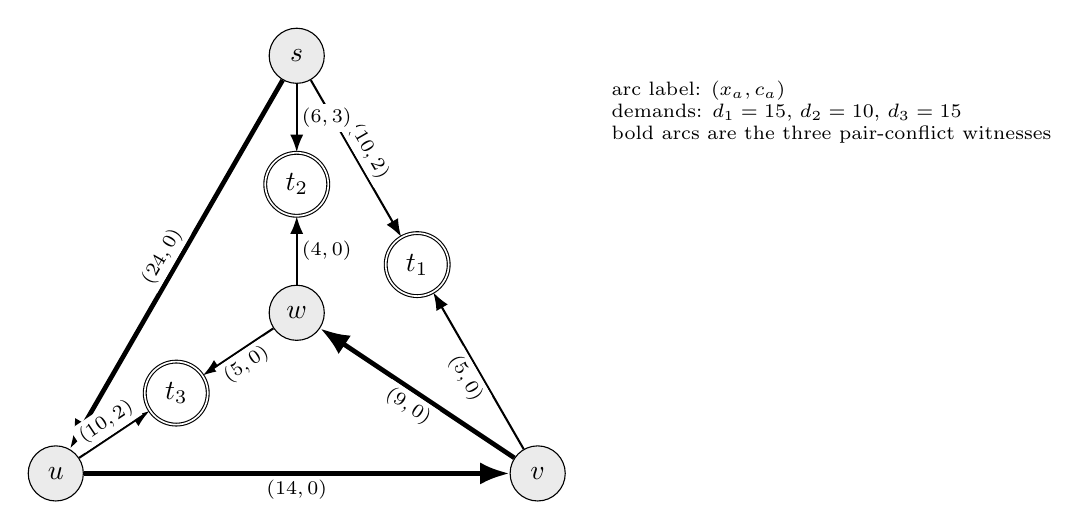
\begin{tikzpicture}[
  scale=1.02,
  >=Latex,
  branch/.style={circle,draw,fill=black!8,minimum size=7mm,inner sep=0pt},
  terminal/.style={circle,draw,double,minimum size=8mm,inner sep=0pt},
  arc/.style={->,line width=0.75pt},
  bottleneck/.style={->,line width=1.7pt},
  lab/.style={fill=white,inner sep=1.5pt,font=\scriptsize}
]
  \node[branch] (s) at (0,3.2) {$s$};
  \node[branch] (u) at (-3,-2) {$u$};
  \node[branch] (v) at (3,-2) {$v$};
  \node[branch] (w) at (0,0) {$w$};

  \node[terminal] (t1) at (1.5,0.6) {$t_1$};
  \node[terminal] (t2) at (0,1.6) {$t_2$};
  \node[terminal] (t3) at (-1.5,-1) {$t_3$};

  \draw[bottleneck] (s) -- node[lab,sloped,above] {$(24,0)$} (u);
  \draw[bottleneck] (u) -- node[lab,below] {$(14,0)$} (v);
  \draw[bottleneck] (v) -- node[lab,sloped,below] {$(9,0)$} (w);

  \draw[arc] (s) -- node[lab,sloped,above] {$(10,2)$} (t1);
  \draw[arc] (v) -- node[lab,sloped,below] {$(5,0)$} (t1);

  \draw[arc] (s) -- node[lab,right] {$(6,3)$} (t2);
  \draw[arc] (w) -- node[lab,right] {$(4,0)$} (t2);

  \draw[arc] (u) -- node[lab,sloped,above] {$(10,2)$} (t3);
  \draw[arc] (w) -- node[lab,sloped,below] {$(5,0)$} (t3);

  \node[align=left,anchor=west,font=\scriptsize] at (3.8,2.5)
    {arc label: $(x_a,c_a)$\\demands: $d_1=15$, $d_2=10$, $d_3=15$\\bold arcs are the three pair-conflict witnesses};
\end{tikzpicture}

\caption{The planar acyclic counterexample.  Arc labels are $(x_a,c_a)$.
The bold arcs are the three pair-conflict witnesses.}
\label{fig:network}
\end{figure}

\begin{lemma}\label{lem:fractional}
The vector $x$ in Table~\ref{tab:arcs} is a feasible fractional flow of cost
$58$.
\end{lemma}
\begin{proof}
A path decomposition is
\[
\begin{array}{lll}
 t_1: &10\text{ on }s t_1,&5\text{ on }suvt_1,\\
 t_2: &6\text{ on }s t_2,&4\text{ on }suvwt_2,\\
 t_3: &10\text{ on }sut_3,&5\text{ on }suvwt_3.
\end{array}
\]
It gives loads $24$ on $su$, $14$ on $uv$, and $9$ on $vw$, with all other
loads as listed.  Equivalently, conservation at $u,v,w$ reads
$24=10+14$, $14=5+9$, and $9=4+5$, while the terminal inflows are
$15,10,15$.  Only the arcs $st_1,st_2,ut_3$ have positive cost, hence
\[
 c^\top x=2\cdot10+3\cdot6+2\cdot10=58.\qedhere
\]
\end{proof}

\subsection{Exhaustive separation}

Each terminal has exactly two directed source--terminal paths:
\[
\begin{array}{lll}
 E_1=st_1, && Z_1=suvt_1,\\
 E_2=st_2, && Z_2=suvwt_2,\\
 E_3=sut_3,&& Z_3=suvwt_3.
\end{array}
\]
The $Z_i$ have zero cost.  Each $E_i$ has total integral cost $30$ after
multiplication by its demand.

\begin{lemma}\label{lem:good-characterization}
An unsplittable routing satisfies $y_a\le x_a+D$ on every arc if and only if it
uses at most one of $Z_1,Z_2,Z_3$.
\end{lemma}
\begin{proof}
If $Z_1$ and $Z_2$ are selected, terminal $3$ uses $su$ on either of its two
paths, so
\[
 y_{su}=15+10+15=40>24+15=39.
\]
If $Z_1$ and $Z_3$ are selected, then
\[
 y_{uv}=15+15=30>14+15=29.
\]
If $Z_2$ and $Z_3$ are selected, then
\[
 y_{vw}=10+15=25>9+15=24.
\]
Thus every pair of zero-cost choices is incompatible.

Conversely, when at most one $Z_i$ is selected, the shared-arc loads obey
$y_{su}\le30<39$, $y_{uv}\le15<29$, and $y_{vw}\le15<24$.  Every other arc is
used by at most one terminal and therefore carries at most $D\le x_a+D$.
\end{proof}

\begin{theorem}\label{thm:dgg-counterexample}
For the instance in Table~\ref{tab:arcs},
\[
 \min\{c^\top y:y\text{ unsplittable},\ y\le x+D\one\}=60>58=c^\top x.
\]
Consequently, Goemans' cost-preserving single-source unsplittable-flow
conjecture is false, even for planar acyclic digraphs.
\end{theorem}
\begin{proof}
By Lemma~\ref{lem:good-characterization}, every feasible routing uses at least
two of $E_1,E_2,E_3$.  Each costs $30$, so the cost is at least $60$.
The routing $(E_1,E_2,Z_3)$ is feasible and costs $60$, proving equality.
Lemma~\ref{lem:fractional} gives the strict comparison with $58$.
\end{proof}

For completeness, Table~\ref{tab:routings} lists all eight routings.  This
also certifies that no unintended path or routing is omitted.

\begin{table}[ht]
\centering
\caption{Exhaustive routing table.}
\label{tab:routings}
\begin{tabular}{@{}cccccl@{}}
\toprule
$t_1$ & $t_2$ & $t_3$ & cost & status & witness\\
\midrule
$E_1$&$E_2$&$E_3$&90&good&--\\
$E_1$&$E_2$&$Z_3$&60&good&--\\
$E_1$&$Z_2$&$E_3$&60&good&--\\
$E_1$&$Z_2$&$Z_3$&30&bad&$vw$: $25>24$\\
$Z_1$&$E_2$&$E_3$&60&good&--\\
$Z_1$&$E_2$&$Z_3$&30&bad&$uv$: $30>29$\\
$Z_1$&$Z_2$&$E_3$&30&bad&$su$: $40>39$\\
$Z_1$&$Z_2$&$Z_3$&0&bad&all three\\
\bottomrule
\end{tabular}
\end{table}

\begin{figure}[ht]
\centering
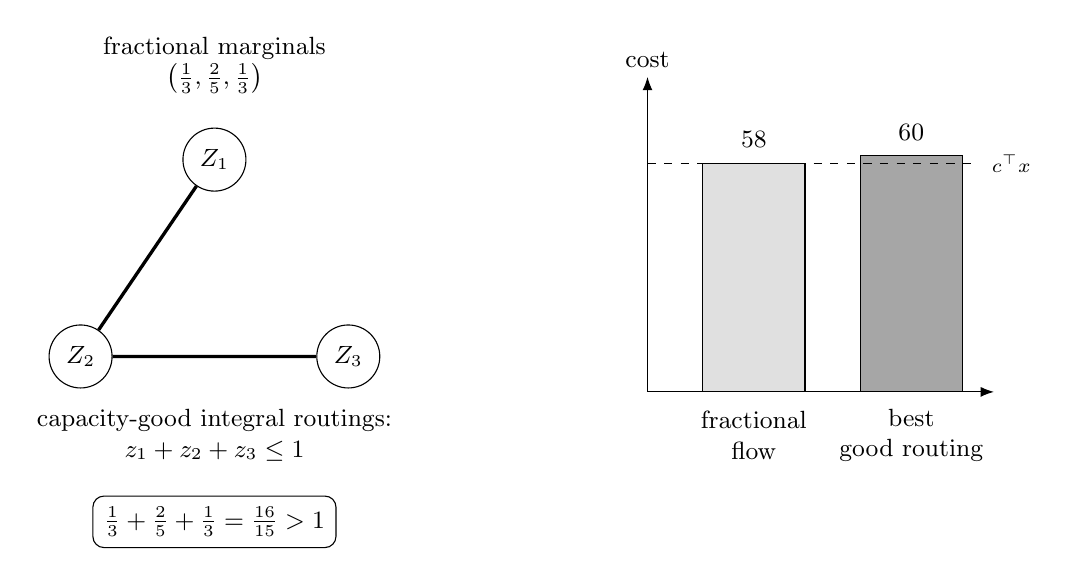
\begin{tikzpicture}[>=Latex,font=\small]
  \begin{scope}[xshift=-3.2cm]
    \node[circle,draw,minimum size=8mm] (z1) at (0,1.8) {$Z_1$};
    \node[circle,draw,minimum size=8mm] (z2) at (-1.7,-0.7) {$Z_2$};
    \node[circle,draw,minimum size=8mm] (z3) at (1.7,-0.7) {$Z_3$};
    \draw[line width=1.2pt] (z1)--(z2)--(z3)--cycle;
    \node[align=center] at (0,-1.7)
      {capacity-good integral routings:\\$z_1+z_2+z_3\le 1$};
    \node[align=center] at (0,3.0)
      {fractional marginals\\$\left(\frac13,\frac25,\frac13\right)$};
    \node[draw,rounded corners,inner sep=4pt] at (0,-2.8)
      {$\frac13+\frac25+\frac13=\frac{16}{15}>1$};
  \end{scope}

  \begin{scope}[xshift=2.3cm,yshift=-1.15cm]
    \draw[->] (0,0)--(0,4.0) node[above] {cost};
    \draw[->] (0,0)--(4.4,0);
    \filldraw[fill=black!12] (0.7,0) rectangle (2.0,2.9);
    \filldraw[fill=black!35] (2.7,0) rectangle (4.0,3.0);
    \node at (1.35,3.2) {$58$};
    \node at (3.35,3.3) {$60$};
    \node[align=center] at (1.35,-0.55) {fractional\\flow};
    \node[align=center] at (3.35,-0.55) {best\\good routing};
    \draw[dashed] (0,2.9)--(4.2,2.9);
    \node[anchor=west,font=\scriptsize] at (4.25,2.9) {$c^\top x$};
  \end{scope}
\end{tikzpicture}

\caption{The structural certificate.  Capacity-good cheap choices form the
stable sets of a triangle, but the fractional cheap-path marginals violate
the triangle facet.  The induced nonnegative separator is the cost gap
$58<60$.}
\label{fig:obstruction}
\end{figure}

\begin{corollary}\label{cor:convex}
The fractional load vector $x$ is not in the convex hull of the unsplittable
load vectors satisfying $y\le x+D\one$.  In particular, it refutes the
cost-and-two-sided-bound conjecture of Morell and Skutella
\cite[Conjecture~2]{MorellSkutella2022}.  It does not refute their costless
existence conjecture with simultaneous upper and lower bounds.
\end{corollary}
\begin{proof}
Every upper-good unsplittable vector has cost at least $60$, whereas
$c^\top x=58$.  The same separator applies to every subset of those vectors,
including the two-sided-good vectors.
\end{proof}

\begin{proposition}\label{prop:positive-cost}
Zero-cost arcs are not essential.  Assign unit cost $1$ to each formerly
zero-cost arc and replace the three positive costs on $st_1,st_2,ut_3$ by
$12,18,12$, respectively.  Then every arc cost is a positive integer, the
fractional cost is $409$, and the minimum upper-good unsplittable cost is
$415$.
\end{proposition}
\begin{proof}
The fractional cost is
\[
 12(10)+18(6)+12(10)+(24+14+5+9+4+5)=409.
\]
The characterization in Lemma~\ref{lem:good-characterization} is unchanged.
The four good-routing costs are $555,420,415,420$, obtained by selecting none
or exactly one of $Z_1,Z_2,Z_3$, respectively.
\end{proof}

\begin{remark}
The underlying undirected graph is a subdivision of $K_4$: suppressing
$t_1,t_2,t_3$ leaves branch vertices $s,u,v,w$.  Hence the example sits
immediately outside the series-parallel class covered by
\citet{AlmoghrabiSkutellaWarode2026}.
\end{remark}

\section{A parametric family and a planar $9/8$ lower bound}

Normalize $D=1$ and retain the same graph.  Let
\[
 d_1=d_3=1,\qquad d_2=b\in(0,1].
\]
In the fractional path decomposition, let the cheap-path probabilities be
$p_1=p_3=r$ and $p_2=q$.  Give each expensive path total integral cost one:
set $c_{st_1}=1$, $c_{st_2}=1/b$, $c_{ut_3}=1$, and all other costs to zero.
The fractional cost is then
\[
 3-(2r+q).
\]

\begin{proposition}\label{prop:parametric}
The parameters define a strict counterexample to the additive-$D$ cost
conjecture whenever
\[
 2r+q>1,\qquad b(1-q)>r,\qquad 2r+bq<1.                 \tag{2}
\]
More generally, every no-more-expensive routing has upper deviation at least
\[
 \min\{1+b(1-q)-r,\ 2-2r-bq\}.                         \tag{3}
\]
\end{proposition}
\begin{proof}
Since $2r+q>1$, the fractional cost is strictly below $2$.  Integral routing
costs are integers, so a no-more-expensive routing uses at most one expensive
path and therefore at least two cheap paths.

The pair $(Z_1,Z_2)$ exceeds the fractional load on $su$ by
$1+b(1-q)-r$.  The pair $(Z_1,Z_3)$ exceeds the fractional load on $uv$ by
$2-2r-bq$.  The pair $(Z_2,Z_3)$ exceeds the fractional load on $vw$ by the
same amount as $(Z_1,Z_2)$.  This proves (3), and the last two inequalities in
(2) make both quantities strictly larger than $D=1$.
\end{proof}

Define $\alpha_{\mathrm{planar}}$ as the infimum of constants $\alpha$ such
that every planar acyclic instance admits an unsplittable $y$ with
$c^\top y\le c^\top x$ and $y_a\le x_a+\alpha D$ for all arcs.

\begin{theorem}\label{thm:nine-eighths}
\[
 \frac98\le \alpha_{\mathrm{planar}}\le2.
\]
Moreover, $9/8$ is the supremum of the lower bounds generated by the symmetric
family above.
\end{theorem}
\begin{proof}
The upper bound is the planar cost theorem of
\citet{TraubVargasKochZenklusen2024}.  For the lower bound take
\[
 b=\frac34,\qquad r=\frac14,\qquad q=\frac12+\eps.
\]
The fractional cost is $2-\eps$, so every no-more-expensive routing uses two
cheap paths.  Each of the three cheap pairs exceeds its corresponding
fractional arc load by
\[
 \frac98-\frac34\eps.
\]
Letting $\eps\downarrow0$ proves $\alpha_{\mathrm{planar}}\ge9/8$.

For optimality within the symmetric family, decrease $q$ to the boundary
$q=1-2r$; this can only increase both expressions in (3).  If $b\ge1/2$, the
two affine expressions are balanced at $r=1-b$, where their common value is
$b(3-2b)$, maximized at $b=3/4$ with value $9/8$.  If $b<1/2$, both relevant
slopes do not yield a value above $1$.  Strict cost separation requires
$q>1-2r$, so $9/8$ is approached but not attained by this normalized family.
\end{proof}

\section{A counterexample to machine-dependent weighted chairman assignment}

We now disprove \citet[Conjecture~19]{LiuReis2026}.  Let
\[
 \eta:=\frac1{1000}.
\]
There are $11$ rows
\[
 B,A_1,H_1,A_2,H_2,\dots,A_5,H_5
\]
and $15$ columns in five consecutive blocks
\[
 J_k,K_k,L_k\qquad(k=1,\dots,5).
\]
Every unspecified fractional entry equals zero and every unspecified weight
equals $\eta$.  In block $k$, the exceptional data are given in
Table~\ref{tab:chairman}.

\begin{table}[ht]
\centering
\caption{One chairman forcing block.}
\label{tab:chairman}
\begin{tabular}{@{}lll@{}}
\toprule
column & nonzero fractional entries & exceptional weights\\
\midrule
$J_k$ & $x_{A_kJ_k}=19/24$, $x_{BJ_k}=5/24$
      & $d_{A_kJ_k}=d_{BJ_k}=1$\\
$K_k$ & $x_{A_kK_k}=1/2$, $x_{H_kK_k}=1/2$
      & $d_{A_kK_k}=1/2$, $d_{H_kK_k}=1$\\
$L_k$ & $x_{A_kL_k}=23/48$, $x_{H_kL_k}=25/48$
      & $d_{A_kL_k}=d_{H_kL_k}=1$\\
\bottomrule
\end{tabular}
\end{table}

Every column sums to one, every column has fractional support two, all weights
are strictly positive, and $D=1$.

\begin{figure}[ht]
\centering
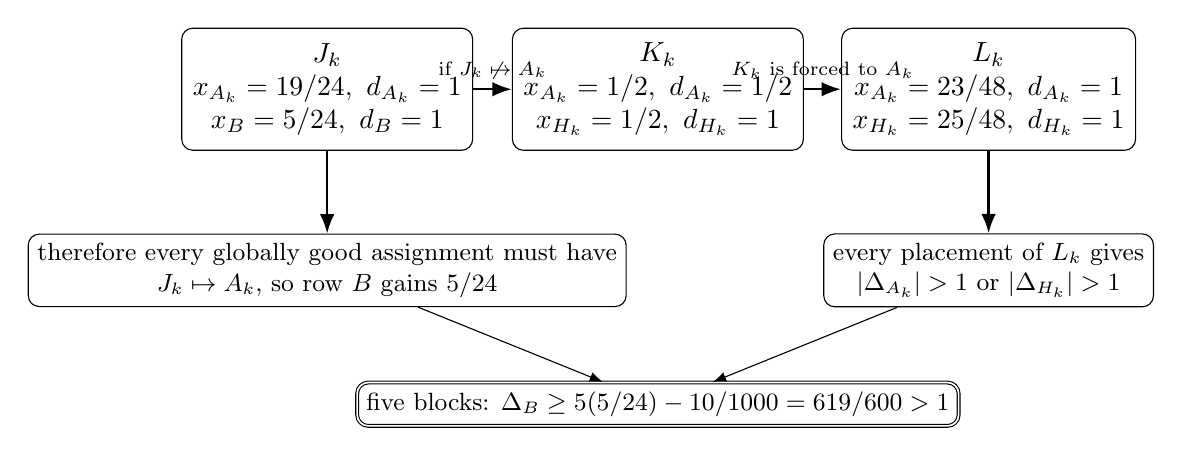
\begin{tikzpicture}[
  >=Latex,
  box/.style={draw,rounded corners,align=center,minimum width=3.0cm,minimum height=1.55cm,inner sep=4pt},
  note/.style={align=center,font=\small}
]
  \node[box] (J) at (0,0) {$J_k$\\$x_{A_k}=19/24,\ d_{A_k}=1$\\$x_B=5/24,\ d_B=1$};
  \node[box] (K) at (4.2,0) {$K_k$\\$x_{A_k}=1/2,\ d_{A_k}=1/2$\\$x_{H_k}=1/2,\ d_{H_k}=1$};
  \node[box] (L) at (8.4,0) {$L_k$\\$x_{A_k}=23/48,\ d_{A_k}=1$\\$x_{H_k}=25/48,\ d_{H_k}=1$};

  \draw[->,line width=0.9pt] (J)-- node[above,font=\scriptsize] {if $J_k\not\mapsto A_k$} (K);
  \draw[->,line width=0.9pt] (K)-- node[above,font=\scriptsize] {$K_k$ is forced to $A_k$} (L);

  \node[note,draw,rounded corners] (bad) at (8.4,-2.3)
    {every placement of $L_k$ gives\\$|\Delta_{A_k}|>1$ or $|\Delta_{H_k}|>1$};
  \draw[->,line width=0.9pt] (L)--(bad);

  \node[note,draw,rounded corners] (force) at (0,-2.3)
    {therefore every globally good assignment must have\\$J_k\mapsto A_k$, so row $B$ gains $5/24$};
  \draw[->,line width=0.9pt] (J)--(force);

  \node[note,draw,double,rounded corners] (repeat) at (4.2,-4.0)
    {five blocks: $\Delta_B\ge 5(5/24)-10/1000=619/600>1$};
  \draw[->] (force)--(repeat);
  \draw[->] (bad)--(repeat);
\end{tikzpicture}

\caption{The three-column detector and five-block accumulator.}
\label{fig:chairman}
\end{figure}

\begin{lemma}\label{lem:forcing}
Every integral assignment satisfying $|\Delta_i(t)|\le1$ for all rows and
prefixes must assign $J_k$ to $A_k$ for every $k=1,\dots,5$.
\end{lemma}
\begin{proof}
Fix $k$.  Before $J_k$, the fresh rows $A_k,H_k$ have zero fractional entries.
At most $3(k-1)\le12$ earlier columns could have been assigned to either row,
and every such off-support assignment contributes $-\eta$.  Thus both current
discrepancies lie in $[-12\eta,0]$.

Suppose $J_k$ is not assigned to $A_k$.  Immediately after $J_k$,
\[
 \Delta_{A_k}\ge-12\eta+\frac{19}{24},
 \qquad
 \Delta_{H_k}\ge-13\eta.
\]
If $K_k$ is not assigned to $A_k$, then $A_k$ is unassigned and gains
$(1/2)(1/2)=1/4$, giving
\[
 \Delta_{A_k}\ge-12\eta+\frac{25}{24}>1.
\]
Hence $K_k$ must be assigned to $A_k$.  Afterwards,
\[
 \Delta_{A_k}\ge-12\eta+\frac{13}{24},
 \qquad
 \Delta_{H_k}\ge-13\eta+\frac12.
\]
If $L_k$ is assigned to $H_k$, then $A_k$ is unassigned and
\[
 \Delta_{A_k}\ge-12\eta+\frac{13}{24}+\frac{23}{48}
 =\frac{49}{48}-12\eta>1.
\]
If $L_k$ is not assigned to $H_k$, then $H_k$ is unassigned and
\[
 \Delta_{H_k}\ge-13\eta+\frac12+\frac{25}{48}
 =\frac{49}{48}-13\eta>1.
\]
Every placement of $L_k$ is impossible, contradicting the assumed prefix
bounds.  Therefore $J_k$ must be assigned to $A_k$.
\end{proof}

\begin{theorem}\label{thm:chairman}
The instance above has no integral assignment satisfying
$|\Delta_i(t)|\le D$ for all rows and prefixes.  Hence Conjecture~19 of Liu
and Reis is false.  The same instance also refutes their unified
Conjecture~21.
\end{theorem}
\begin{proof}
By Lemma~\ref{lem:forcing}, every hypothetical good assignment sends every
$J_k$ to $A_k$.  Row $B$ is therefore unassigned on all five $J$ columns and
gains $5/24$ on each.  The only possible decreases on row $B$ occur if one of
the ten $K/L$ columns is assigned off support to $B$, each contributing only
$-\eta$.  At the final prefix,
\[
 \Delta_B\ge5\left(\frac5{24}\right)-10\eta
 =\frac{619}{600}>1=D.
\]
This contradiction proves the first claim.  Since no assignment at all obeys
the bounds, certainly no support-preserving assignment obeys them; thus the
instance also refutes the stronger unified statement.
\end{proof}

\begin{remark}
The common-column-weight theorem of \citet{LiuReis2026} is not affected.  The
counterexample uses machine dependence essentially: an off-support assignment
has weight $\eta$, while the detector can place weight $1$ on the row whose
fractional contribution must be protected.
\end{remark}

\section{Structural interpretation and significance}

For the flow instance, let $z_i=1$ indicate that terminal $i$ uses its cheap
path $Z_i$.  Lemma~\ref{lem:good-characterization} says that capacity-good
integral routings satisfy the triangle stable-set facet
\[
 z_1+z_2+z_3\le1.
\]
The fractional cheap-path marginals are
\[
 \left(\frac13,\frac25,\frac13\right),
 \qquad
 \frac13+\frac25+\frac13=\frac{16}{15}>1.
\]
Thus the cost vector is not an ad hoc numerical choice; it is a nonnegative
separator for a violated integral-hull inequality.  This also explains the
convex-decomposition failure in Corollary~\ref{cor:convex}.

The first conjecture was explicit in the minimum-cost literature by 2002 and
was described as a $25$-year-old conjecture in the recent series-parallel work
\cite{AlmoghrabiSkutellaWarode2026}.  Its failure matters because the additive
$D$ bound without costs is optimal and remains valid; the example isolates the
incompatibility between that sharp congestion guarantee and exact cost
preservation.  The planar $9/8$ family begins a quantitative replacement
question between the new lower bound and the known factor $2$.

The chairman counterexample addresses a much newer conjecture, posed in the
November 2025 preprint and January 2026 conference publication of
\citet{LiuReis2026}.  Its role is different: it identifies machine-dependent
weights as a genuine boundary for the weighted chairman phenomenon, even when
the fractional support is only two per column and the instance uses just three
weight values $\{1,1/2,1/1000\}$.

\section{Verification and reproducibility}

The accompanying repository contains JSON instances and three independent
checks.  The standard-library script \texttt{verify\_dgg.py} enumerates every
directed source--terminal path and all eight unsplittable routings, reconstructs
the fractional load vector from its path decomposition, and checks both the
$58$--$60$ certificate and the all-positive $409$--$415$ variant.
The script \texttt{verify\_chairman\_certificate.py} checks every displayed
rational inequality.  Finally, \texttt{verify\_chairman\_milp.py} scales all
data by $6000$ and asks an independent HiGHS mixed-integer model whether any
assignment obeys every prefix bound; the model is infeasible.

The discovery and drafting process used GPT-5.6 Pro for mathematical
exploration, checking, code generation, and language editing.  The AI system
is not an author.  The submitting human author is responsible for independent
verification, attribution, disclosure, and all claims in the final paper.

\paragraph{Provenance.}
The flow counterexample of Sections~3--4 (the seven-vertex instance, its
positive-cost variant, the Morell--Skutella corollaries, and the parametric
$9/8$ family) originated in an earlier portion of a shared AI research
conversation conducted by a third party, before the present repository owner's
involvement.  It is reproduced here for completeness only and is \emph{not}
claimed as a contribution of the repository owner.  This combined manuscript
must therefore not be submitted as-is; the repository owner's separable
contribution is the chairman counterexample of Section~5, available as a
standalone manuscript in
\texttt{2026-rounding-counterexamples/papers/chairman-counterexample.tex}.
See \texttt{PROVENANCE\_AUDIT.md} at the repository root.

\section{Conclusion}

A seven-vertex planar DAG suffices to separate the sharp additive
Dinitz--Garg--Goemans bound from exact cost preservation.  The obstruction is
a triangle facet, and its symmetric scaling yields a planar lower bound of
$9/8$ on any replacement cost-preserving theorem.  Separately, an eleven-row,
fifteen-column detector refutes the machine-dependent weighted-chairman
extension.  Both examples suggest that small violated facets and repeated
forcing gadgets are useful design principles for locating the exact boundary
of weighted rounding theorems.

\bibliographystyle{plainnat}
\bibliography{references}

\end{document}
